%
% File emnlp2020.tex
%
%% Based on the style files for ACL 2020, which were
%% Based on the style files for ACL 2018, NAACL 2018/19, which were
%% Based on the style files for ACL-2015, with some improvements
%%  taken from the NAACL-2016 style
%% Based on the style files for ACL-2014, which were, in turn,
%% based on ACL-2013, ACL-2012, ACL-2011, ACL-2010, ACL-IJCNLP-2009,
%% EACL-2009, IJCNLP-2008...
%% Based on the style files for EACL 2006 by 
%%e.agirre@ehu.es or Sergi.Balari@uab.es
%% and that of ACL 08 by Joakim Nivre and Noah Smith

\documentclass[11pt,a4paper]{article}
\usepackage[hyperref]{emnlp2020}
\usepackage{times}
\usepackage{latexsym}
\renewcommand{\UrlFont}{\ttfamily\small}
\usepackage{todonotes}
\usepackage{enumitem}
\usepackage{amssymb}
\usepackage{tabularx}
\usepackage{subcaption}
\usepackage{booktabs}
\usepackage{multirow}

% This is not strictly necessary, and may be commented out,
% but it will improve the layout of the manuscript,
% and will typically save some space.
\usepackage{microtype}

%\aclfinalcopy % Uncomment this line for the final submission
%\def\aclpaperid{***} %  Enter the acl Paper ID here

%\setlength\titlebox{5cm}
% You can expand the titlebox if you need extra space
% to show all the authors. Please do not make the titlebox
% smaller than 5cm (the original size); we will check this
% in the camera-ready version and ask you to change it back.

\newcommand\BibTeX{B\textsc{ib}\TeX}

\title{Spot The Bot}

\author{First Author \\
  Affiliation / Address line 1 \\
  Affiliation / Address line 2 \\
  Affiliation / Address line 3 \\
  \texttt{email@domain} \\\And
  Second Author \\
  Affiliation / Address line 1 \\
  Affiliation / Address line 2 \\
  Affiliation / Address line 3 \\
  \texttt{email@domain} \\}

\date{}

\begin{document}
\maketitle
\begin{abstract}

\end{abstract}

\section{Introduction}
Evaluation is a crucial step in the development cycle of dialogue systems, which is very cost-and time-intensive and often not reproducible. This problem is especially pronounced for conversational dialogue systems (i.e. chit-chat bots), which work on open domains and do not have a clearly defined goal, which can be measured. This not only slows down the development of novel approaches but it also makes it hard to reliably recreate the evaluation. 
There are several open problems: 
\begin{itemize}
\item  Human-bot conversations are costly to obtain and they often suffer from low quality. Low quality dialogues are the result of the limited capabilities of the algorithms, which are specialized on one domain and the fact that humans do not adhere to the distribution in which the model has been trained. Furthermore, the cognitive strain on the annotators is increased when they have to both converse with the bot and then rate the conversation \cite.
\item Human ratings are less costly to obtain but they often suffer from low agreement scores. Furthermore, these ratings are hard to reproduce and not necessarily stable across different executions. 
\item Current offline evaluations do not take into account the multi-turn character of conversations. Often, the evaluation is performed on a static context (e.g. sampled from a test set) and a generated response utterance of the bot under consideration. 
\item There is a general lack of automation of the evaluation procedure. Most automated metrics do not correlate to human judgements \cite{}, or are unstable.
\end{itemize}

In this work, we present \emph{Spot The Bot} a cost-and-time efficient evaluation methodology, which can be used to reliably discriminate different dialogue strategies. \emph{Spot The Bot} is based on the observation that conversational dialogue systems are trained on human-human conversations, and thus, the dialogue systems should be evaluated in their ability to mimic human behaviour. This idea is related to the Turing Test, where the goal is that a bots' behaviour is indistinguishable from human behaviour.
\emph{Spot The Bot} works by letting two bots converse with eachother and letting crowdworkers decide for each entity in the conversation if it is a human or a bot. Since we assume that in most cases the bots are identified as such, we add a time component so that the discriminating criterion is: for which dialogue system can hide its non-humanity the longest. 



\section{Spot The Bot}
\subsection{Overview}
% figure
%----------------------------------------------------------------------------
\begin{figure*}[h]
	\begin{center}
        \begin{tabular}{@{}c@{}}
		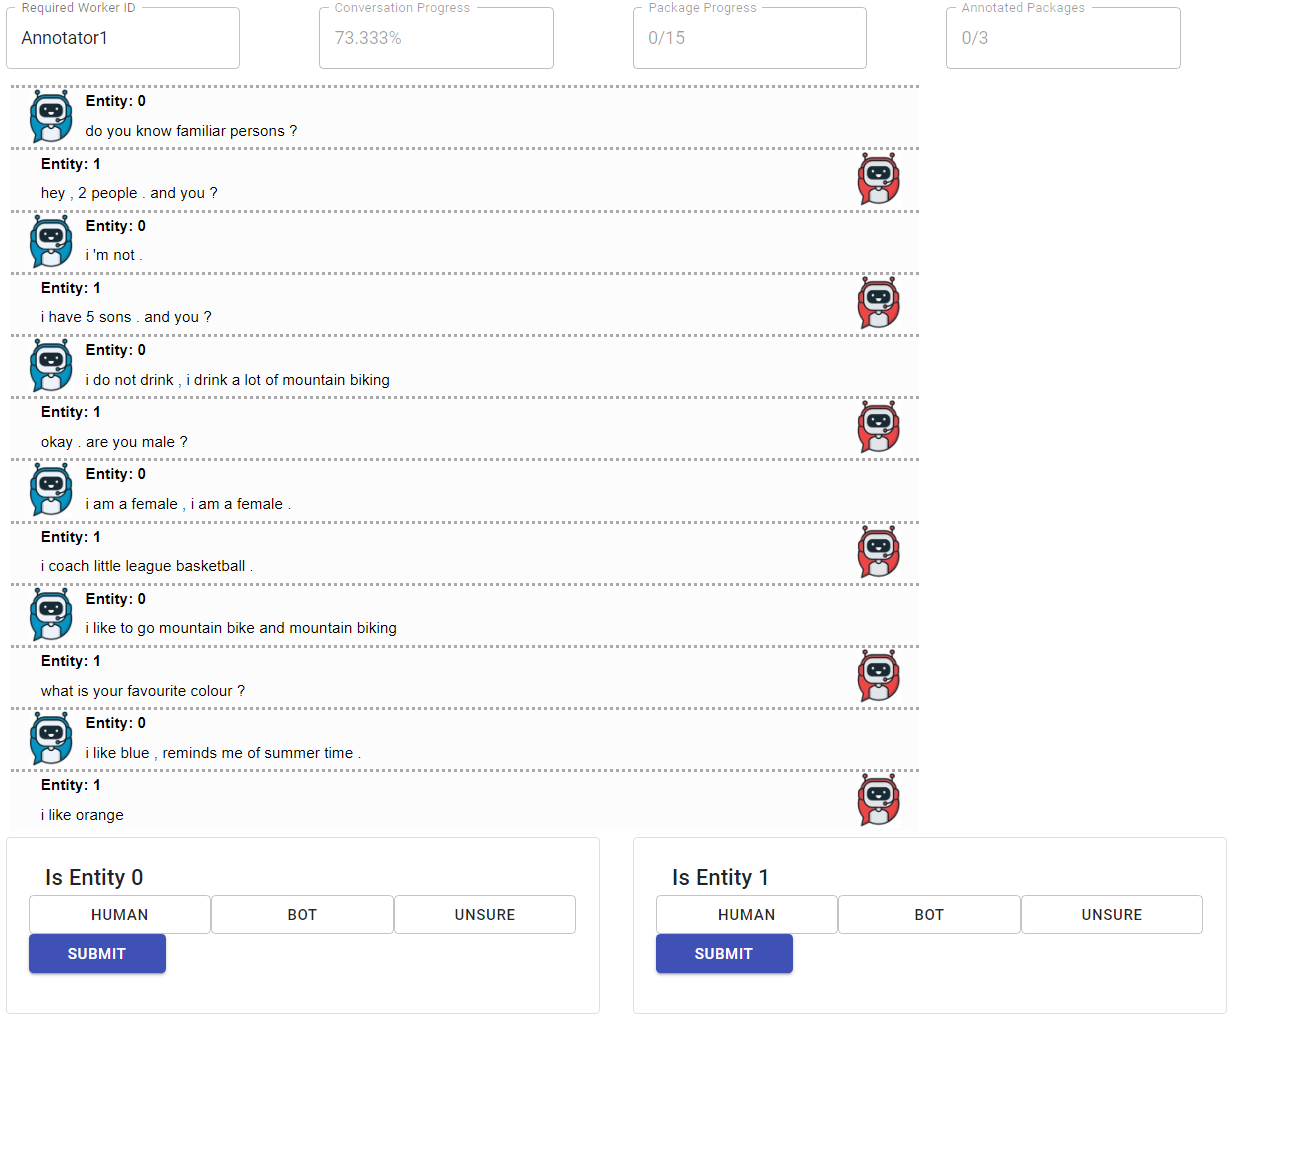
\includegraphics[width=0.45\textwidth]{figures/AnnotationTool1.png} 
		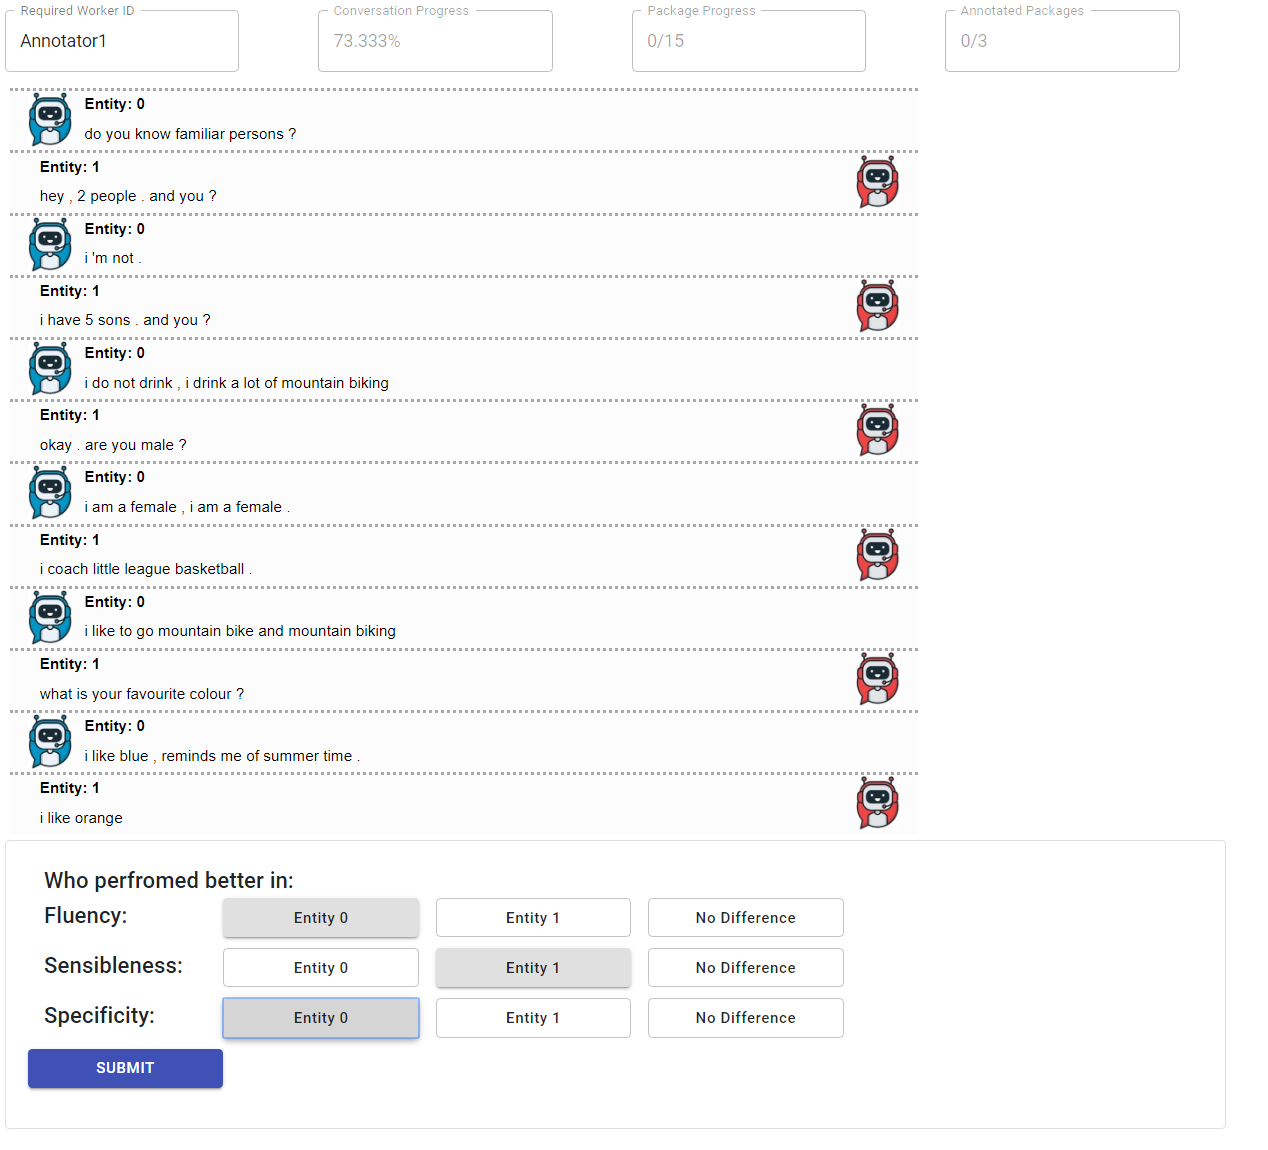
\includegraphics[width=0.45\textwidth]{figures/AnnotationTool2.png}
       \end{tabular}
	\end{center}\vspace{-3mm}
	\captionof{figure}{The annotation tool. Left is the decision about the nature of each entity. Right is the decision with regard to the features. }
\label{fig:tool}
\end{figure*}
%----------------------------------------------------------------------------
Assume that there is a pool of N conversational dialogue systems $\{B_1, ..., B_N\}$, which is to be ranked. For instance, when a novel dialogue strategy is to be compared against existing strategies. For each pair of bots, a set of conversations is sampled by letting the bots talk to each other, where $S_{ij}$ denotes the set of conversations between $B_i$ and $B_j$. Each conversation is defined as a sequence of exchanges $e_0, ..., e_N$, where each exchange consists of two turns, one per entity $e_i = \{t_0^{e_i}, t_1^{e_i}\}$. 
Spot The Bot defines the task of letting human crowdworkers read a conversation and decide for each entity in the conversation if it is a human or a bot. This setting alone would not yield satisfying results for two reasons: first, most conversational dialogue systems are not yet human-like enough to fool humans, second, the corwdworkers would soon realize that all conversations are among bots, thus, classifying all entities as bots. 
For the first issue, we add a time component: we show the conversation at different stages: $e_0, ..., e_i$. The bots are then differentiated not only by their ability to fool humans but also by how long they are able to pass as a human or at least not be spotted as a bot. For the second issue, we add conversations among humans into the pool, as well as conversations between humans and bots. These serve two purposes: first, as distractors, so that the crowdworkers cannot classify all as bots, and second, as a upper bound on how often humans are mistakenly classified as bots.
Additionally, we ask to state which bot performed better with regards to certain features: fluency, sensibleness, and specificity as defined in \cite{}. 
We apply three different analysis on the annotated data: fooling rate (i.e. how often was the bot classified as a human), pair-wise ranking (rank the bots based on pair-wise comparisons from the annotated conversations), and survival analysis (i.e. probability of survival at each exchange).

\subsection{Setting}
%ToDo cite and explain a bit more
We applied Spot The Bot on three different domains: Personachat, Dailydialogues, and Empathetic Dialouges. Each of these domains is based on conversations between two humans in different settings. For each of the domains, we prepared a pool of bots to be ranked. 


\paragraph{Bot-Bot Conversations.} For each pair of bots $B_i$, $B_j$ in the pool, we sample $|S_{ij}| = 15$ conversations. In order to increase the variety of dialogues in $S_{ij}$, the initial context of the conversation is sampled from the test set of the domain. The initial context is not shown to the crowdworkers. 
\paragraph{Segmentation.} In order to simulate the time component, we show the conversations at different stages $e_0, ..., e_i$, where we chose different sets of values for $i$ depending on the domain\footnote{We experimented with letting crowdworkers decide themselves when to decide the exchange at which they were sure that an entity in the conversation is a bot or a human. However, this approach introduced too much unwanted behaviour.}. Each segment is annotated by different annotators to avoid that one annotator sees the same conversation multiple times. 
\paragraph{Annotation.} The generated bot-bot conversations, a set of randomly sampled human-human conversation from the training material, and human-bot conversations are presented to crowdworker to be rated. The crowdworker are presented with a conversation segment, and have to decide for each conversation participant if it is a human or a bot. There is a option for "unsure" as well, since we are interested in cases when the annotators are sure about their decision. 
\paragraph{Features.} After the decision, the crowdworkers are asked to decide for each of the three features (i.e. fluency, specificity, and sensibleness) which entity performed better in each of these features. 

\subsection{Setup}

\begin{table}[h!]
\vspace{-1mm}
\begin{center}
\begin{small}
\resizebox{.45\textwidth}{!}{
\begin{tabular}{l||cccl} 
\hline
%\abovespace
\textsc{Domain Name} & \textsc{\#Dialogues} &  \textsc{Average Exchanges} &  \textsc{$|B|$} & \textsc{Domain Description}\\
\hline 
\textsc{Dailydialog}  &     13118     &  &   5  & Dialogues based on daily communication              \\
\textsc{Epathetic Dialogues} &    25000   & 1.65 &   5   &     Dialogues with emotion labels            \\
\textsc{Personachat}    & 10907   &  &   6   & Dialogues based on predefined profiles          \\
\hline
\end{tabular}
}
\end{small}
\\~\\
  \vspace{1mm}
\end{center}
\caption{Overview of the domains}
\label{table:domain-overview}
\end{table}

\paragraph{Domains.} We train our systems on three different domains:  Dailydialog, Empathetic Dialogues, and Personachat. The training data for each of these domains are conversation about humans (see Table \ref{table:domain-overview} for Overview). 

\paragraph{Systems.}  

\paragraph{Amazon Mechanical Turk.} We recruited paid crowdworkers from Amazon Mechanical Turk (AMT). In order to avoid that the results are dependent on the performance of a single crowdworker, we designed a HIT as a batch of 20 conversations and each worker was only allowed to work on three batches. We designed the batches so that two segments of the same conversations never appear in the same batch, and each batch contains different segments of different conversations.  

\paragraph{Human-Bot Conversations.} Ideally, this approach works without relying on human-bot conversations, which are costly to obtain and often very noisy if not executed with care. We show that our approach works without the need of human-bot conversations, by comparing the results of the \emph{Spot The Bot}  annotation procedure with and without human-bot conversations. 


\section{Results}

We evaluate the results from different perspectives. We compute the fooling rates, that is the number of times a bots behaviour was able to pass as a human. In order to take into account the time component, we apply a survival analysis, which computes the probability of survival at each point in time. Finally, we exploit the pairwise conversations to generate a ranking based on pairwise ratings. 

\subsection{Fooling Rates}
The fooling rate is defined as the ratio of annotations where a dialogue system was classified as being a human. 

\subsection{Survival Analysis}


\subsection{Ranking}
From the pairwise ratings, we generate a ranking by interpreting it as a game between two bots. Intuitively, the bot that is able to fool a human earlier or hide its non-humanity longer, can be considered the better bot. More precisely, we count each annotation at each segment $s_j = e_0, ... , e_{i_j}$ as one game. Since each segment is annotated $M$ times, and there $S$ segments per conversation, we have $M*S$ games per conversation. We first compute the winner for each game, then we compute the winner for each segment, and finally, we compute the overall winner for the conversation. The winner of a single game is determined by the annotation, with following points: $\textit{human}=2, \textit{unsure}=1$, and $\textit{bot}=0$. The winner of the segment is determined by the bot that won the most of the $M$ games within a segment. In case of a tie, the winner is determined by the amount of points. The winner of the overall game is determined by who won the most games. However, this would not take into account that longer segments are harder, as the probability of being exposed as a bot is higher. The winner of segment $s_j$ receives $log(i_j)$ points, and the bot with the most points over all segments wins the game. Thus, a bot, that lost in earlier segments but won in later segments wins the game.

\begin{table}[h!]
\vspace{-1mm}
\begin{center}
\begin{small}
\resizebox{.25\textwidth}{!}{
\begin{tabular}{l|cccl} 
\hline
%\abovespace
\textsc{} & \textsc{BR} &  \textsc{HF} &  \textsc{S2} & \textsc{DR}\\
\hline 
\textsc{BR} & - & 0.60 & 0.6 & 0.66  \\
\textsc{HF} & 0.40 & - & 0.46 & 0.60  \\
\textsc{S2} & 0.40 & 0.33 & - & 0.60  \\
\textsc{DR} & 0.20 & 0.26 & 0.2 & - \\
\end{tabular}
}
\end{small}
\\~\\
  \vspace{1mm}
\end{center}
\caption{Win Rates for Empathetic Dialogues.}
\label{table:domain-overview}
\end{table}

 

\section{AutoJudge}

\section{Case Study: Reranking ConvAI2}

\section{Discussion}

\section{Related Work}


\section{Conclusion and Future Work}

\section*{Acknowledgments}

\bibliography{emnlp2020}
\bibliographystyle{acl_natbib}

\appendix

\section{Appendices}
\label{sec:appendix}

\end{document}
